% TODO:
% - decide whether to submit a companion JOSS paper
% - huh? http://adsabs.harvard.edu/abs/2014ApJ...790..127B
% - When Hogg's Gaussian Product Refactor note is on Arxiv, check the referenced
%   equation numbers in the Appendix against the submitted version!

\documentclass[modern]{aastex63}
% \documentclass[twocolumn]{aastex63}
\usepackage{amsmath}

% Load common packages
\usepackage{microtype}  % ALWAYS!
\usepackage{amsmath}
\usepackage{amsfonts}
\usepackage{amssymb}
\usepackage{booktabs}

\usepackage{graphicx}
\usepackage{color}

% Numbers:
\newcommand{\nsources}{\ensuremath{232,531}}
\newcommand{\Kmin}{K_{\rm min}}
\newcommand{\Kminval}{512}
\newcommand{\nbinary}{\ensuremath{19,635}}

\graphicspath{{figures/}}
% \definecolor{cbblue}{HTML}{3182bd}
% \usepackage{hyperref}
% \definecolor{linkcolor}{rgb}{0.02,0.35,0.55}
% \definecolor{citecolor}{rgb}{0.45,0.45,0.45}
% \hypersetup{colorlinks=true,linkcolor=linkcolor,citecolor=citecolor,
%             filecolor=linkcolor,urlcolor=linkcolor}
% \hypersetup{pageanchor=true}

\newcommand{\documentname}{\textsl{Article}}
\newcommand{\sectionname}{Section}
\renewcommand{\figurename}{Figure}
\newcommand{\equationname}{Equation}
\renewcommand{\tablename}{Table}

% Missions
\newcommand{\project}[1]{\textsl{#1}}

% Packages / projects / programming
\newcommand{\package}[1]{\textsl{#1}}
\newcommand{\acronym}[1]{{\small{#1}}}
\newcommand{\github}{\package{GitHub}}
\newcommand{\python}{\package{Python}}
\newcommand{\emcee}{\project{emcee}}

% For referee
\newcommand{\changes}[1]{{\color{red} #1}}

% Stats / probability
\newcommand{\given}{\,|\,}
\newcommand{\norm}{\mathcal{N}}

% Maths
\newcommand{\dd}{\mathrm{d}}
\newcommand{\transpose}[1]{{#1}^{\mathsf{T}}}
\newcommand{\inverse}[1]{{#1}^{-1}}
\newcommand{\argmin}{\operatornamewithlimits{argmin}}
\newcommand{\mean}[1]{\left< #1 \right>}

% Unit shortcuts
\newcommand{\msun}{\ensuremath{\mathrm{M}_\odot}}
\newcommand{\kms}{\ensuremath{\mathrm{km}~\mathrm{s}^{-1}}}
\newcommand{\mps}{\ensuremath{\mathrm{m}~\mathrm{s}^{-1}}}
\newcommand{\pc}{\ensuremath{\mathrm{pc}}}
\newcommand{\kpc}{\ensuremath{\mathrm{kpc}}}
\newcommand{\kmskpc}{\ensuremath{\mathrm{km}~\mathrm{s}^{-1}~\mathrm{kpc}^{-1}}}
\newcommand{\dayd}{\ensuremath{\mathrm{d}}}

% Misc.
\newcommand{\bs}[1]{\boldsymbol{#1}}

% Astronomy
\newcommand{\DM}{{\rm DM}}
\newcommand{\feh}{\ensuremath{{[{\rm Fe}/{\rm H}]}}}
\newcommand{\df}{\acronym{DF}}
\newcommand{\logg}{\ensuremath{\log g}}
\newcommand{\Teff}{\ensuremath{T_{\textrm{eff}}}}

% TO DO
\newcommand{\todo}[1]{{\color{red} TODO: #1}}

\newcommand{\dr}[1]{\acronym{DR}#1}
\newcommand{\apogee}{\acronym{APOGEE}}
\newcommand{\sdss}{\acronym{SDSS}}
\newcommand{\sdssiv}{\acronym{SDSS-IV}}
\newcommand{\thejoker}{\project{The~Joker}}

\shorttitle{Stellar companions in APOGEE}
\shortauthors{Price-Whelan et al.}

\begin{document}\sloppy\sloppypar\raggedbottom\frenchspacing % trust!

\title{Binary companions to APOGEE DR16 stars: \\
       Catalog of XX systems}

\author[0000-0003-0872-7098]{Adrian~M.~Price-Whelan}
\affiliation{Center for Computational Astrophysics, Flatiron Institute,
             Simons Foundation, 162 Fifth Avenue, New York, NY 10010, USA}
\email{aprice-whelan@flatironinstitute.org}
\correspondingauthor{Adrian M. Price-Whelan}

% \author[0000-0003-2866-9403]{David~W.~Hogg}
% \affiliation{Max-Planck-Institut f\"ur Astronomie,
%              K\"onigstuhl 17, D-69117 Heidelberg, Germany}
% \affiliation{Center for Cosmology and Particle Physics,
%              Department of Physics,
%              New York University, 726 Broadway,
%              New York, NY 10003, USA}
% \affiliation{Center for Data Science,
%              New York University, 60 Fifth Ave,
%              New York, NY 10011, USA}
% \affiliation{Flatiron Institute,
%              Simons Foundation,
%              162 Fifth Avenue,
%              New York, NY 10010, USA}

% \author[0000-0003-4996-9069]{Hans-Walter~Rix}
% \affiliation{Max-Planck-Institut f\"ur Astronomie,
%              K\"onigstuhl 17, D-69117 Heidelberg, Germany}

\author{Others}

\begin{abstract}
% Context
Binary star systems provide key context and constraints for nearly all subfields in astrophysics, yet precise inferences about binary star populations typically rely on just hundreds of stars nearest to the sun.
Detailed knowledge of binary star population properties is therefore
% Aims
Contemporary stellar surveys already observe large numbers of stars
% Methods
We have a big hammer
% Results
We produce posterior samplings assuming...SB1 and two-body systems...
We also produce a catalog of binary systems...we select on evidence or parameter estimation...
% Conclusions
Binaries all over HR diagram...but we find ??
We find interesting low-mass and high-mass systems...
\end{abstract}

\keywords{}


\section{Introduction} \label{sec:intro}

A better understanding the population of binary stars throughout our galaxy is important for all aspects of astrophysics. For example, ... stellar-mass binary black hole mergers to stellar populations in high-redshift galaxies \citep[e.g.,][]{Breivik:BAAS, Rix:BAAS}.

We need to understand the population statistics of stellar multiplicity and their variations with stellar type, chemistry, and dynamical environment.

This problem spans a wide range of timescales, wavelengths, and many current and near-future stellar surveys (Gaia, APOGEE, LAMOST, SDSS-V, etc.) have the capacity to deliver samples of binary stars and stellar companions orders of magnitude larger than are presently known, throughout all stages of stellar evolution.
The dream: combine all if this and learn ...
This has only been comprehensively done for a sample of a few hundred stars in solar neighborhood.

As a step towards large-scale population inference, we focus here on multi-epoch spectroscopic data from the APOGEE surveys.
The challenge: data are often sparse, most individual systems are not determined uniquely.
We have machinery to generate full samplings over orbital parameters for radial velocity data, under the assumptions listed in The Joker paper (SB1, etc.).
We run this sampler on all of APOGEE DR16 with some quality cuts and release the resulting catalog of posterior samples, along with some summary metadata for unimodal / uniquely determined orbits.

We use these samples to infer the companion period-eccentricity distribution over the HR diagram as an initial demonstration of hierarchical inference.


\section{Data} \label{sec:data}

We primarily use spectroscopic data from data release 16 (\dr{16}) of the
\apogee\ surveys (\citealt{Majewski:2017, Abolfathi:2017, DR16}).
\apogee\ is a component of the Sloan Digital Sky Survey IV (\sdssiv;
\citealt{Gunn:2006, Blanton:2017}) and its main goal is to survey the chemical
and dynamical properties of stars across much of the Milky Way disk by obtaining
high-resolution ($R \sim 22,500$) infrared ($H$-band) spectroscopy of hundreds
of thousands of stars.
The primary survey targets are selected with simple color and magnitude cuts,
but the survey uses fiber-plugged plates that leads to extremely nonuniform
coverage of the Galactic stellar distribution (see, e.g., Figure~1 in
\citealt{DR16}).

\dr{16} is the first \sdss\ data release to contain \apogee\ data observed with
a duplicate of the \apogee\ spectrograph on the 2.5m du Point telescope at Las
Campanas Observatory, providing access to targets in the southern hemisphere.
For the first time, this data release also contains calibrated stellar
parameters for dwarf stars.
These two facts mean that \dr{16} contains nearly $3\times$ more sources with
calibrated stellar parameters than the previous public data release, \dr{14}
(see Section~4 of \citealt{DR16} for many more details about \apogee\ \dr{16}).

Most \apogee\ stars are observed multiple times in a set of time-resolved
``visits'' that are combined before the \apogee\ \todo{ASPCAP} determines
stellar parameters and chemical abundances for each source.
While the visit spectra naturally provide time-domain velocity information about
sources (thus enabling searches for massive companions), studying stellar
multiplicity is not the primary goal of the survey:
The cadence and time baseline for a typical \apogee\ source is primarily
governed by trying to schedule a set number of visits determined by
signal-to-noise thresholds for the faintest targets in a given field.
A consequence of this strategy is that the time resolution and number of visits
for the vast majority of \apogee\ sources in \dr{16} is not sufficient for fully
determining companion orbital properties, as illustrated below.
Still, the large number of targets in \apogee\ and the dynamic range in stellar
and chemical properties offers an exciting opportunity to study the
\emph{population} of binary star systems as a function of these intrinsic
properties, even if most individual systems are poorly constrained.
We have previously developed tools to enable such studies \citep{thejoker}, as
summarized in \sectionname~\ref{sec:methods} below.
Here, we describe quality cuts we apply to the \apogee\ \dr{16} catalogs before
proceeding, and modifications to the visit-level velocity uncertainties to
account for the fact that they are generally underestimated by the \apogee\ data
reduction pipeline.


\subsection{Quality cuts and defining a parent sample}

The primary goal of this \documentname\ is to produce a catalog of posterior
samplings in Keplerian orbital parameters for all high-quality \apogee\ sources
in \dr{16} with multiple, well-measured radial velocities.
We therefore impose a set of quality cuts to sub-select \apogee\ \dr{16} sources
by rejecting sources or visits using the following \apogee\
bitmasks\footnote{https://www.sdss.org/dr16/algorithms/bitmasks/}:
\begin{itemize}
    \item Source-level (\texttt{allStar}) \texttt{STARFLAG} must not contain
    \texttt{VERY\_BRIGHT\_NEIGHBOR}, \texttt{SUSPECT\_RV\_COMBINATION} (bitmask
    value: 65544)
    \item Source-level (\texttt{allStar}) \texttt{ASPCAPFLAG} must not contain
    \texttt{TEFF\_BAD}, \texttt{LOGG\_BAD}, \texttt{VMICRO\_BAD},
    \texttt{ROTATION\_BAD}, \texttt{VSINI\_BAD} (bitmask value: 1141309440)
    \item Visit-level (\texttt{allVisit}) \texttt{STARFLAG} must not contain
    \texttt{VERY\_BRIGHT\_NEIGHBOR}, \texttt{SUSPECT\_RV\_COMBINATION},
    \texttt{LOW\_SNR}, \texttt{PERSIST\_HIGH}, \texttt{PERSIST\_JUMP\_POS},
    \texttt{PERSIST\_JUMP\_NEG} (bitmask value: 78360)
\end{itemize}
These bitmasks are designed to remove the most obvious data reduction or
calibration failures that would directly impact the visit-level radial velocity
determinations.
However, we later impose a stricter set of quality masks when showing results in
\sectionname~\ref{sec:TODO}.
After applying the above masks, we additionally reject any source with $<3$
visits.
Our final parent sample contains \nsources\ unique sources, selected from the
$437,485$ unique sources in all of \apogee\ \dr{16}.
Of the $\approx$$200,000$ sources removed, the vast majority were dropped
because they had $<3$ visits ($\approx$$17,000$ were removed by the quality
cuts).

% Notebook: Figure-DR16-statistics.ipynb
\begin{figure}[!t]
\begin{center}
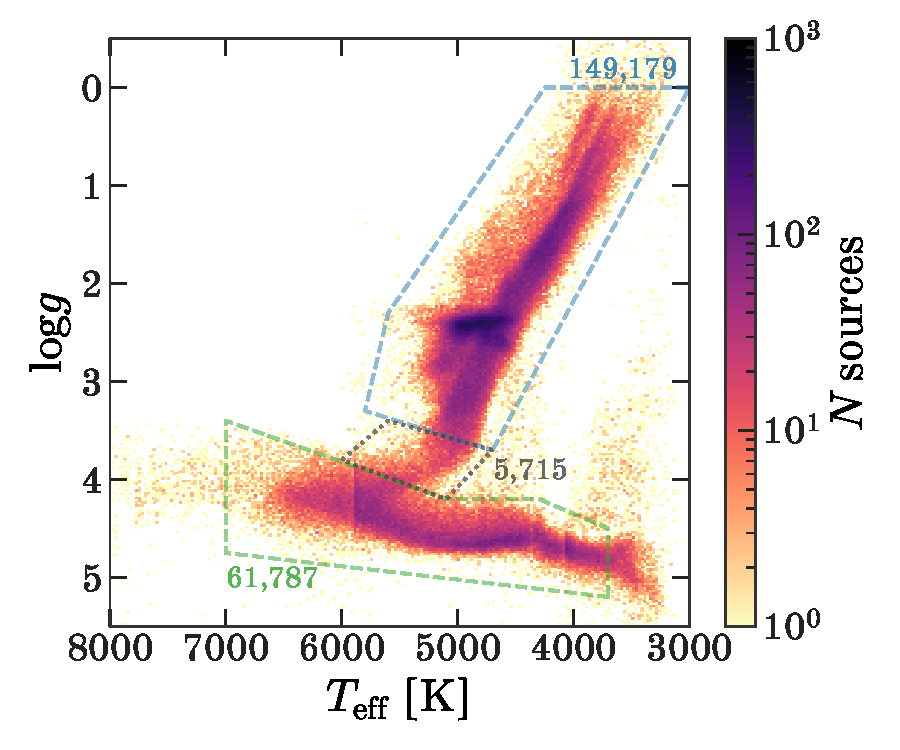
\includegraphics[width=0.7\textwidth]{specHR.pdf}
\end{center}
\caption{%
Two spectroscopic stellar parameters---effective temperature, $T_{\rm eff}$, and
log-surface gravity, $\log g$---of \apogee\ \dr{16} sources that pass our
quality cuts; These sources represent our ``parent sample.''
The pixel coloring indicates the number of sources in each bin of stellar
parameters.
The outlined regions roughly identify the red giant branch (upper polygon,
blue), subgiant branch (middle polygon, black), and (FGK-type) main sequence
(lower polygon, green).
The numbers next to each selection polygon indicate the number of sources in
each.
\label{fig:specHR}
}
\end{figure}

% Notebook: Figure-DR16-statistics.ipynb
\begin{figure}[!t]
\begin{center}
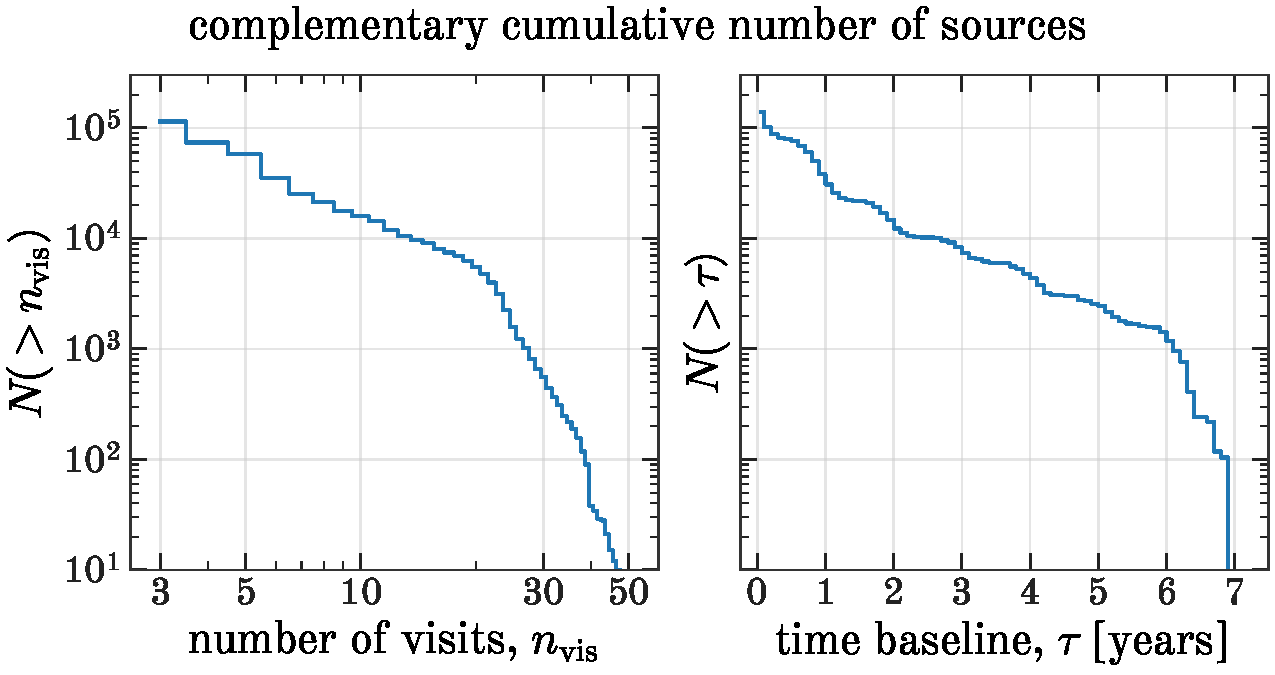
\includegraphics[width=1\textwidth]{visitstats.pdf}
\end{center}
\caption{%
Some statistics of \apogee\ \dr{16} visits.
\textbf{Left:} The number of sources with more than a given number of visits,
$n_{\rm vis}$.
While $\approx$$50\%$ of sources have 3 visits, ($114,263$, $57,593$, $15,862$)
sources have $> (3, 5, 10)$ visits, respectively.
A very small number of sources have $>50$ visits.
\textbf{Right:} The number of sources with a time baseline, $\tau$, longer than
given (on the horizontal axis).
While $\approx$$50\%$ of sources have a time baseline $\tau \lesssim 56~{\rm
day}$, ($88,737$, $9,743$) sources have $\tau > (100, 1000)~{\rm days}$.
\label{fig:visitstats}
}
\end{figure}

Figure~\ref{fig:specHR} shows the number of sources in our parent sample---i.e.
\apogee\ sources with 3 or more visits that pass the quality cuts described
above---as a function of spectroscopic stellar parameters $T_{\rm eff}$,
effective temperature, and $\log g$, log-surface gravity.
While the majority of sources appear to be giant-branch stars ($>150,000$), a
substantial number of main sequence stars are present ($>60,000$) thanks to the
\apogee\ data reduction pipeline improvements for \dr{16}.
Figure~\ref{fig:visitstats} shows some statistics about the time coverage of the
visits for sources in our parent sample.
About half of the sources have a small number of visits spread over a small time
baseline: $50\%$ of sources have $<5$ visits over $<100~{\rm days}$.
About $7\%$ of sources ($15,366$) have $\geq 10$ visits over $\geq 100~{\rm
days}$.


\subsection{Visit velocity uncertainty calibration} \label{sec:visitcalib}

The significance of apparent radial velocity variations, especially when
considering low-mass or long-period companions, will depend strongly on the
correctness of the visit velocity measurement errors.
However, the catalog-level \apogee\ visit velocity errors (\texttt{VRELERR} in
the \texttt{allVisit} file) are known to be underestimated
\citep[e.g.,][]{Cottaar:2014}.
Here, we adopt the relation defined in Brown et al. (in prep.) to scale up the
visit velocity errors
\begin{equation}
    \sigma_v^2 = (3.5\,(\texttt{VRELERR})^{1.2})^2 + (0.072~\kms)^2 \label{eq:verr}
\end{equation}
where $\sigma_v$ is the adopted visit velocity error for a given visit, and
\texttt{VRELERR} is the uncertainty reported in the \apogee\ \dr{16} catalog.
This effectively applies a floor to the visit velocity errors of $72~\mps$ and
globally increases the error values by a multiplicative factor.


\section{Methods} \label{sec:methods}

As illustrated above, a large number of sources in \apogee\ \dr{16} have few
visits that span a short time baseline.
For most sources, we therefore expect that even if visit-level radial velocity
variations are detected with high significance, the companion orbital parameters
will be very uncertain---i.e. the posterior probability distribution function
(\pdf) over orbital parameters will generally be multi-modal with many
modes of comparable integrated probability \citep[e.g.,][]{thejoker}.
Still, in unison, or within the context of a hierarchical model that utilizes
the individual posterior samplings, the combination of all of these individually
weakly-constrained binary star orbits should still provide information about the
population of binary stars.
We have previously defined and implemented a custom Monte Carlo sampler for
precisely this problem: \thejoker\ \citep{thejoker}.
\thejoker\ is designed to deliver converged posterior samplings over Keplerian
orbital parameters given radial velocity observations, even when the
observations are sparse or very noisy.
We have previously applied \thejoker\ to \apogee\ \dr{14}
\citep{Price-Whelan:2018} and, by making some conservative selections with the
returned samplings, released a catalog of over $5,000$ binary star systems;
This \documentname\ and companion catalog is a successor to this previous work.

In this \documentname, as with previous work, we use a parametrization of the
two-body problem in which the radial velocity, $v$, of an observed star in a
binary system (referred to as the \emph{primary}, even if it is less massive
than its companion) can be expressed as:
\begin{equation}
    v(t) = K \, \zeta(t \,;\, P, e, \omega, M_0, t_0) + v_0 \label{eq:kepler}
\end{equation}
where $K$ and $v_0$ are linear parameters (in time $t$).
The other parameters---period $P$, eccentricity $e$, argument of periastron
$\omega$, reference time $t_0$, and mean anomaly at reference time $M_0$---enter
through the nonlinear function
\begin{equation}
    \zeta(t \,;\, P, e, \omega, M_0, t_0) = \cos\left(f + \omega\right) + e\,\cos\omega \label{eq:zeta}
\end{equation}
where $f$ is the true anomaly, and we always set the reference time, $t_0$, to
the minimum observation time for a given set of radial velocity observations.

\subsection{Updates to \thejoker}
\label{sec:joker-update}

Since our initial paper defining \thejoker, we identified a conceptual error in
the assumptions made about the prior over the linear parameters ($K$, $v_0$) in
\citet{thejoker}.
We previously assumed that adopting a sufficiently broad, Gaussian prior over
the linear parameters meant that we could ignore an explicit definition of this
prior.
In particular, this allowed us to drop any terms related to the prior over these
parameters in the marginal likelihood expression \citep[\equationname~11
in][]{thejoker}.
This assumption is not correct, and can lead to unexpected behavior when applied
to data that are very noisy or have a small time baseline compared to the
samples of interest.
We have rewritten the expression for the marginal likelihood that underlies
\thejoker\ in Appendix~\ref{app:marginal-likelihood}, based on the notation in
\cite{Hogg:2020}.

Another issue with the assumption in the original implementation of \thejoker\
is that the prior over the velocity semi-amplitude, $K$, was identical at all
period and eccentricity values.
This implicitly implies vastly different prior beliefs about the companion mass
as a function of orbital period: For example, a zero-mean Gaussian prior on $K$
with a standard-deviation of $30~\kms$ transforms to reasonable prior beliefs
about companion mass at periods around $1~{\rm year}$, but gives substantial
prior probability to companion masses $>100~\msun$ at periods $>10^4~\dayd$.
We therefore, by default, adopt a new (also Gaussian) prior on the
semi-amplitude with a variance, $\sigma^2_K$, that scales with the
period and eccentricity such that
\begin{equation}
    \sigma^2_K = \sigma^2_{K, 0} \, \left(\frac{P}{P_0}\right)^{-2/3} \,
        \left(1 - e^2\right)^{-1} \label{eq:sigK}
\end{equation}
where $\sigma_{K, 0}$ and $P_0$ are additional hyperparameters that must be
specified.
This new prior on $K$ has the advantage that it, at fixed primary mass, has a
fixed form in companion mass that does not depend on period or eccentricity.

We have also made a number of improvements to the Python implementation of the
sampler.\footnote{https://github.com/adrn/thejoker}
For example, the prior distributions over all parameters are now specified as
\texttt{pymc3} \citep{Salvatier2016} distribution objects, meaning that the
priors over the nonlinear Keplerian parameters ($P$, $e$, $\omega$, and $M_0$;
see \citealt{thejoker}) are now fully customizable.
Using \texttt{pymc3} also enables compatibility with more efficient Markov Chain
Monte Carlo methods such as Hamiltonian Monte Carlo (HMC), which is useful for
seamlessly transitioning from generating posterior orbit samples with \thejoker\
to HMC when the system parameters are highly constrained (as discussed below).


\section{Running \thejoker\ on all of \apogee\ \dr{16}} \label{sec:rundr16}

For each of the \nsources\ sources in the parent catalog of sources selected
from \apogee\ \dr{16} (\sectionname~\ref{sec:data}), we run \thejoker\
\citep{thejoker} generate posterior samplings over the Keplerian orbital
parameters, plus an additional per-source uncertainty or ``jitter'' parameter
that is added in quadrature to the (adjusted) \apogee\ visit velocity
uncertainties (see above).
We start by generating a cache of $100,000,000$ prior samples for the nonlinear
parameters generated from the prior \pdf\ summarized in
\tablename~\ref{tbl:prior} (top rows).
For each source, we iteratively read random blocks of samples out of this cache,
evaluate the marginal likelihood, and rejection sample to produce posterior
samplings in the nonlinear parameters.
We repeat this iterative process until we reach the total number of samples in
the cache, or until we obtain a requested number of prior samples, $\Kmin$; This
is an arbitrary parameter that we set to $K_{\rm min} = \Kminval$ for this work.
In practice, this is done by parallelizing the sampling (over sources) and takes
about 8 hours to run on 720 cores on our local compute cluster (at the Flatiron
Institute).

After the procedure described above, the sources have one of two stages of
completion: Sources either have $\Kmin = \Kminval$ posterior samples (\todo{XX}
sources) and are complete, or $\Kmin < \Kminval$ posterior samples (\todo{XX}
sources) and more samples are needed.
For sources that require more samples, these can be split again into two
classes: Sources with unimodal samplings in period, and sources with multi-modal
samplings (following the criteria described in \citealt{thejoker}).
For incomplete sources with unimodal samplings (\todo{XX} sources), we use the
samples returned from \thejoker\ to initialize Hamiltonian Monte Carlo (HMC) to
continue generating posterior samples.
We use \texttt{pymc3} with the \emph{No-U-Turn Sampler} (NUTS; \citealt{NUTS}),
using the dense mass matrix tuning prescription implemented in
\texttt{exoplanet} \citep{exoplanet:exoplanet} and run 4 chains in parallel,
each for 1000 tuning steps and 4000 steps subsequently.
We use these 4 chains and \texttt{pymc3} to compute the Gelman-Rubin convergence
statistic, $\hat{R}$ \citep{Gelman:1992}, for each parameter for each source; If
$\hat{R} < 1.1$ for all parameters, we down-sample to \Kminval\ samples and mark
that source as MCMC-completed.
If the HMC sampling fails (e.g., chains diverge substantially), we fall back to
the sampling from \thejoker---this generally only happens for data with serious
systematic issues (e.g., one outlier visit velocity with an unreasonable
velocity measurement).

At this point, we now have \Kminval\ posterior samples in the parameters listed
in \tablename~\ref{tbl:prior} for \todo{XX} \apogee\ sources; These are released
as a component of the \sdss\ Value-Added Catalog (VAC).

\begin{table}[h]
    \centering
    \setlength{\tabcolsep}{0.75em} % for the horizontal padding
    \begin{tabular}{ r l p{6cm} }
    \toprule
    \textbf{parameter} & \textbf{prior} & \textbf{description} \\
    \toprule
    \multicolumn{3}{l}{\footnotesize \textsl{nonlinear parameters}}\\
    \hline
    $P$ & $\ln P \sim \mathcal{U}(2, 16384)~\textrm{day}$ & period \\
    $e$ & $e \sim \textrm{Beta}(0.867, 3.03)$ & eccentricity \\
    $t_0$ & fixed (minimum time) & reference time \\
    $M_0$ & $M_0 \sim \mathcal{U}(0, 2\pi)~\textrm{rad}$ & mean anomaly at reference time \\
    $\omega$ & $\omega \sim \mathcal{U}(0, 2\pi)~\textrm{rad}$ & argument of pericenter \\
    $s$ & $\ln s \sim \mathcal{N}(\mu_y, \sigma_y^2)$ & extra ``jitter'' added in quadrature to each visit velocity error \\
    \hline
    \multicolumn{3}{l}{\footnotesize \textsl{linear parameters}}\\
    \hline
    % $K$ & $K \sim \mathcal{N}(0, \sigma_{K}^2)~\kms$ & velocity semi-amplitude, where $\sigma_K$ is given by \equationname~\ref{eq:sigK} with $\sigma_{K,0} = 30~\kms$ and $P_0 = 365~\dayd$. \\
    $K$ & $K \sim \mathcal{N}(0, \sigma_{K}^2)~\kms$ & velocity semi-amplitude, where $\sigma_K$ is given by \equationname~\ref{eq:sigK}\\
    & $\sigma_{K,0} = 30~\kms$ & (see \equationname~\ref{eq:sigK})\\
    & $P_0 = 365~\dayd$ & (see \equationname~\ref{eq:sigK})\\
    $v_0$ & $v_0 \sim \mathcal{N}(0, \sigma_{v_0}^2)~\kms$ & system barycentric velocity \\
    & $\sigma_{v_0} = 100~\kms$ & \\
    \bottomrule
    \end{tabular}
    \caption{Summary and description of parameters and prior \pdf s. $\textrm{Beta}(a, b)$ is the
    beta distribution with shape parameters $(a, b)$, $\mathcal{U}(a, b)$ the
    uniform distribution over the domain $(a, b)$, and $\mathcal{N}(\mu,
    \sigma^2)$ is the normal distribution with mean $\mu$ and variance
    $\sigma^2$.}
    \label{tbl:prior}
\end{table}

\subsection{Assumptions, caveats, and known failures}
\label{sec:caveats}

The assumptions that underlie the sampling procedure described above are
enumerated in \sectionname~3.1 in \cite{Price-Whelan:2018}.
We therefore briefly rephrase the most important implications of these
assumptions as a set of caveats and points of caution for any users of the
posterior samplings generated here.

First, despite allowing for a per-source, additive (in variance) extra
uncertainty parameter ($s$ in \tablename~\ref{tbl:prior}), we are very sensitive
to outliers, or, more generally, any visit velocities with strongly non-Gaussian
noise properties.
In \apogee, this might occur for blended sources, multiple-star systems with
more than one star that contribute significantly to infrared flux, or sources
with stellar parameters very beyond the grid of template spectra
\citep{Nidever:2015}.
Second, the adopted prior \pdf\ over systemic velocities, $v_0$, is reasonable
for considering all \apogee\ sources (i.e., for a mixture of kinematically
disk-like and halo-like sources), but may lead to biased posterior samplings for
sources in globular clusters or dwarf galaxies.
For such systems, it would be safer to re-run \thejoker\ with specialized priors
over systemic velocity for each individual host system.
Finally, in this work, we assume that all systems are binary systems, so triples
or higher-order stellar multiplets will generally have incorrect samplings.
In future work, we will generate samplings for systems that are consistent with
being hierarchical triple-star systems, but this is beyond the scope of this
general-use catalog.


\section{A catalog of binary stars} \label{sec:catalog}

For some science cases and exploration (as demonstrated below), it is useful to
filter these stars to generate catalogs of systems with likely companions.
This requires making some decisions and imposing hard cuts on the samplings
returned by the above procedure.
However, most of the orbital parameter samplings for most sources are highly
uncertain and multi-modal, and it is therefore not possible to define simple
cuts on physical parameters like companion mass to produce a simple catalog.
In the previous iteration of this work \citep{Price-Whelan:2018}, we defined
cuts based on percentiles computed from the distribution of $\ln K$ values after
comparing to running the same pipeline on a control sample of data generated
with purely Gaussian noise properties and time information taken from the
\apogee\ \dr{14} visits.
Here, we use both a selection based on the posterior samples in $K$ and based on
a likelihood ratio comparing the Keplerian orbit model assumed by \thejoker\
with a (robust) constant-velocity model for each source.

Following \citet{Price-Whelan:2018}, we again compute the 1st-percentile values
of the posterior samples in $\ln K$ for each source and refer to these values as
$P_{1\%}(\ln K)$.
We again also generate a simulated control sample of data to assess
contamination when making selections using this quantity.
For each \apogee\ source in our parent sample, we take the maximum \textsl{a
posteriori} sample returned from the procedure defined above and subtract the
orbit computed from this sample from the visit velocity data.
We then re-run \thejoker\ on all of the residual data, and compute $P_{1\%}(\ln
K)$ for each star in the control sample.
We find that $<5\%$ of the control sample pass a cut of $P_{1\%}(\ln K) > 0$
(i.e., a conservative cut to require that sources have a velocity semi-amplitude
$> 1~\kms$).

For each \apogee\ source, after generating the posterior samplings, we compute
and store the maximum (over posterior samples) \emph{unmarginalized}
log-likelihood value for the Keplerian orbit model, i.e., for one source with
$N$ visit velocity measurements $v_n$ at times $t_n$,
\begin{equation}
    \ln \hat{L}_1 = \sum_n^N \ln \mathcal{N}(v_n \given
        v(t_n \,;\, \bs{\theta}_{\mathrm{max}}), \sigma_n^2)
\end{equation}
where $\sigma_n$ are the adjusted visit velocity errors
(\equationname~\ref{eq:verr}) and $v(\cdot)$ is given by
\equationname~\ref{eq:kepler} and is evaluated using the parameters for the
maximum likelihood posterior sample, $\bs{\theta}_{\mathrm{max}}$.

For each source, we then also compute the maximum log-likelihood value for the
visit data under a model that assumes that the visit velocities are drawn from a
constant velocity with Gaussian uncertainties but allowing for up to a $20\%$
outlier fraction (over visits); We refer to this model as a \emph{robust
constant-velocity} model for the visit velocities.
Using the same notation for the visit velocity data as above, the likelihood
under this model is given by
\begin{equation}
    L_2 = \prod_n^N \left[(1-f) \, \mathcal{N}(v_n \given \mu_v, \sigma_n^2)
        + f\, \mathcal{N}(v_n \given \mu_v, \sigma_n^2 + \Sigma) \right]
\end{equation}
where $f$ is the outlier fraction, $\mu_v$ is the constant-velocity value, and
$\Sigma$ is the variance of the outlier model component (assumed to be large).
We optimize this likelihood using the BFGS \citep{BFGS} algorithm with bounds on
the parameters such that $f \in (0, 0.2)$, $\mu_v \in (-500, 500)~\kms$, and
$\Sigma \in (0, 3000)~(\kms)^2$.
We store the optimized log-likehihood value of the robust constant-velocity
model and refer to this as $\ln \hat{L}_2$

We define a catalog of binary star systems based on the posterior samplings
generated from \thejoker\ by selecting sources for which
\begin{align}
    P_{1\%}(\ln K) &> 0\\
    (\ln \hat{L}_1 - \ln \hat{L}_2) &> 4.6 \quad . \label{eq:binary-cuts}
\end{align}
The cut on the log-likelihood ratio comes from the (arbitrary) constraint that
the maximum Kepler model likelihood should be $>100$ times the maximum robust
constant-velocity likelihood value.
Of the \nsources\ total sources in our parent sample, \nbinary\ sources pass the
selection above.

% Notebook: Figure-binary-examples.ipynb
\begin{figure}[!t]
    \begin{center}
    % \includegraphics[width=1\textwidth]{example-binaries.pdf}
    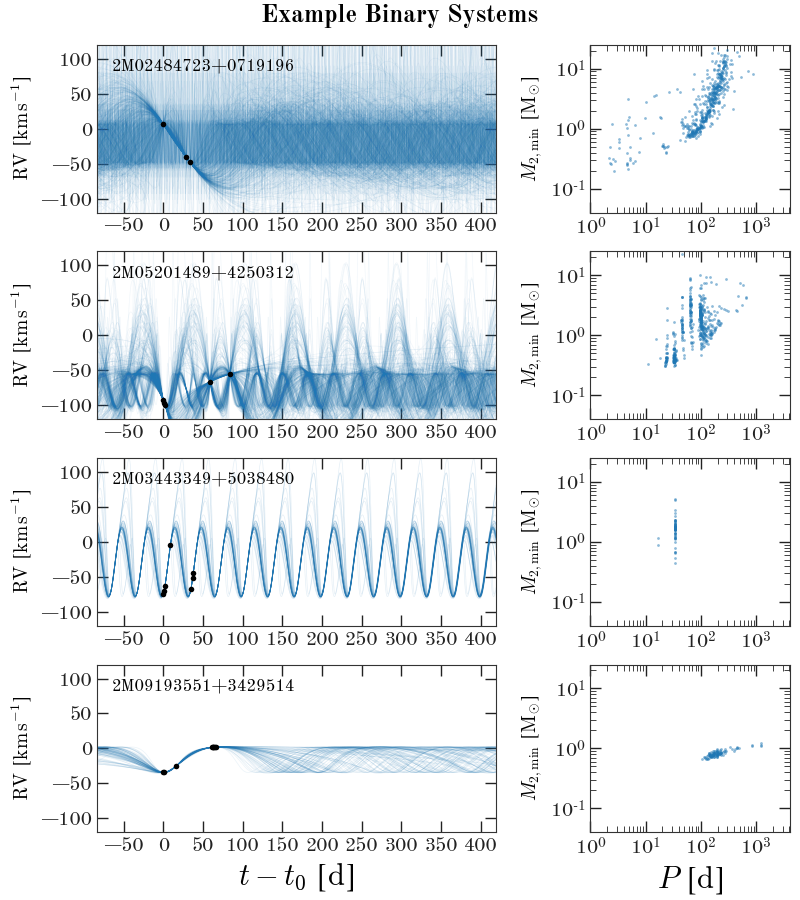
\includegraphics[width=0.8\textwidth]{example-binaries-placeholder.png}
    \end{center}
    \caption{%
    Example binary star systems that pass the selection and are included in the
    catalog released here.
    Each row is an \apogee\ source (indicated on the left panel).
    Left panels show the visit velocity data (black markers; error bars are
    typically smaller than the marker) and radial velocity orbits computed from
    the posterior samples (blue lines).
    Right panels show the same samples in period $P$ and minimum companion mass
    \mtwomin.
    \label{fig:binary-examples}
    }
\end{figure}

\figurename~\ref{fig:binary-examples} shows some examples of systems that passed
the selection above and are considered binary star systems; Each row is a
different \apogee\ source.
The left column of panels show the radial velocity data (black markers) for
randomly-chosen sources with (3, 5, 7, 9) visits (from top to bottom), and the
blue lines show radial velocity orbits computed from the posterior samplings
generated by \thejoker.
The right column of panels show the same posterior samples (blue markers), but
in a projection of the parameter space (period $P$ and minimum companion mass,
\mtwomin).
To compute \mtwomin, we use the posterior samplings from \thejoker\ along with
primary stellar masses computed by \citet{starhorse2019} by sampling over the
reported uncertainties on prior mass (assuming a Gaussian noise distribution on
primary mass).

% Notebook: Figure-binary-fraction.ipynb
\begin{figure}[!t]
    \begin{center}
    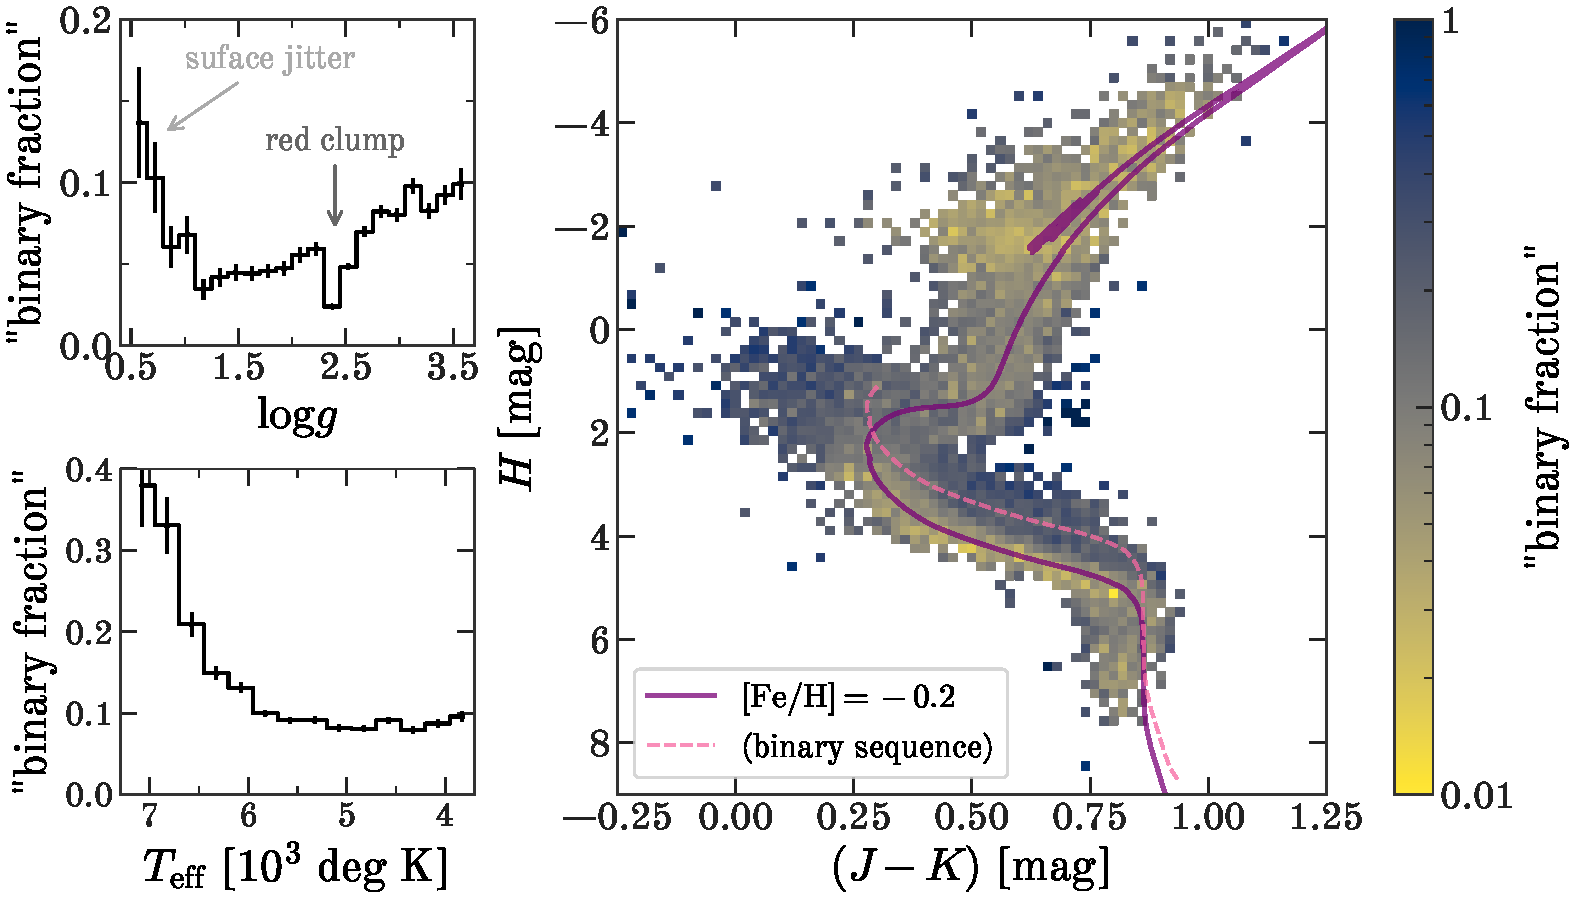
\includegraphics[width=0.85\textwidth]{binary-fraction.pdf}
    \end{center}
    \caption{%
    \textbf{Upper left:} TODO
    \textbf{Lower left:} TODO
    \textbf{Right:} The extinction-corrected \acronym{2MASS} color-magnitude
    diagram (CMD) for all \apogee\ sources, colored by the fraction of sources
    identified as binary-star systems (\sectionname~\ref{sec:catalog}).
    Solid lines show \acronym{MIST} isochrones for a $5~\mathrm{Gyr}$ with
    $\feh = -0.5$ (orange) and $\feh = 0.5$ (red), to bracket the range of
    metallicities of typical \apogee\ sources; Dashed lines (with the same
    coloring) indicate the equal-mass binary sequence for main sequence stars,
    %
    The panels in this figure are meant to be illustrative and should only be
    compared in a relative sense.
    \label{fig:binary-CMD}
    }
\end{figure}

% TODO: left panels use the selections from figure 1
\figurename~\ref{fig:binary-CMD} (right) shows a near-infrared, binned
color-magnitude diagram for all \apogee\ sources in the sample considered here.
Each pixel is colored by the ratio of the number of binary star systems
identified by the selections defined above (\equationname~\ref{eq:binary-cuts})
over the total number of sources in the parent sample; Pixels with fewer than
four stars in the parent sample are nulled.
The two solid lines show $5~\mathrm{Gyr}$ \acronym{MIST} isochrones \citep{MIST}
with metallicities indicated in the figure legend.
The dashed lines show the equal-mass binary sequences for these two isochrones,
$0.75~\mathrm{mag}$ above the main sequence: Note that, as expected, the binary
fraction is higher in this region of the CMD, and is higher towards younger /
more massive main sequence stars.
Note also that the red clump (around $(J-K) \approx 0.6$, $H \approx -1.8$) has
a \emph{low} binary fraction: This is likely a manifestation of engulfment, as
these stars have already been up the giant branch and would therefore have
consumed any companions with periods less than a few hundred days.
The dearth of binary systems near the red clump is also apparent when
visualizing the total binary fraction as a function of surface gravity, as shown
in the top left panel of \figurename~\ref{fig:binary-CMD}.
The bottom left panel shows the same as a function of effective temperature
(as a proxy for the mass of the primary): The binary fraction appears to
increase for more massive stars.

This ignores survey selection effects, inclination, and selection biases
introduced by the cuts we made to identify binary star systems.


% TODO: what about bimodal samplings, or samplings with small range in ln-period?


\section{Results} \label{sec:results}

\subsection{Gold sample}

Figure: ...

\subsection{Interesting low and high mass companions}


\subsection{Hierarchical inference of the long-period eccentricity distribution}


\subsection{Circularization}


\subsection{Engulfment}


% \section{Inferring shit with a hierarchical model} \label{sec:Pe}

% \begin{align}
%     z &= \ln\,P\\
%     \bs{\theta} &= (z, e)\\
%     \bs{\alpha} &= (k, z_0, \alpha_0)\\
%     p(\bs{\theta} \given \bs{\alpha}) &= p(z) \, p(e \given z)\\
%     p(z) &= \norm\left(z \given \mu_z, \sigma_z^2 \right)\\
%     p(e \given z) &= \alpha(z) \, p_1(e) + (1-\alpha(z)) \, p_2(e)\\
%     f(z\,;\,k,z_0) &= \frac{1}{1 + e^{-k\,(z - z_0)}}\\
%     \alpha(z \,;\, k, z_0, \alpha_0) &= (1-\alpha_0) \, f(z \,;\, k, z_0) + \alpha_0\\
%     p_1(e) &= B(e \given a_1, b_1)\\
%     p_2(e) &= B(e \given a_2, b_2)
% \end{align}

% \begin{align}
%     p(D \given \bs{\alpha}) &= \int \dd\bs{\theta} \,
%         p(D \given \bs{\theta}) \, p(\bs{\theta} \given \bs{\alpha})\\
%     &\approx \frac{\mathcal{Z}}{K} \sum_k^K
%         \frac{p(\bs{\theta}_k \given \bs{\alpha})}
%             {p(\bs{\theta}_k \given \bs{\alpha}_0)}\\
%     \bs{\theta}_k &\sim p(\bs{\theta} \given D, \bs{\alpha}_0)
% \end{align}

% - Period, eccentricity distributions
% - Mass-ratio distribution
%      - Use C,N abundances for RGB and logg, teff, fe/h for main sequence
%      - Calibrate against asteroseismology / APOKASC


% Lars: "Any idea of the incidence of stars which did an engulfment on their way UP the RGB from the Luminosity of the clump to that of the RGB TIP? "

% Note: some or all of these may be broken out into separate papers!

% \subsection{Companions along the RGB}
% Compare RGB vs. RC - see engulfment?
%
% \subsection{Brown dwarfs}
% So many!
%
% \subsection{Binary population statistics}
% Simple hierarchical inference?
%
% \subsection{TRGB asteroseismology}
%
% \subsection{Binary star populations in open clusters}
%
% \subsection{Binary star populations in globular clusters}

% Ack: Lars Bildsten

\acknowledgements

It is a pleasure to thank
Lars Bildsten (KITP)
Dan Foreman-Mackey (Flatiron),
...
% We thank the anonymous referee for constructive comments that improved this
% manuscript.

Funding for the Sloan Digital Sky Survey IV has been provided by the Alfred P.
Sloan Foundation, the U.S. Department of Energy Office of Science, and the
Participating Institutions. SDSS-IV acknowledges support and resources from the
Center for High-Performance Computing at the University of Utah. The SDSS web
site is www.sdss.org.

SDSS-IV is managed by the Astrophysical Research Consortium for the
Participating Institutions of the SDSS Collaboration including the Brazilian
Participation Group, the Carnegie Institution for Science, Carnegie Mellon
University, the Chilean Participation Group, the French Participation Group,
Harvard-Smithsonian Center for Astrophysics, Instituto de Astrof\'isica de
Canarias, The Johns Hopkins University, Kavli Institute for the Physics and
Mathematics of the Universe (IPMU) / University of Tokyo, Lawrence Berkeley
National Laboratory, Leibniz Institut f\"ur Astrophysik Potsdam (AIP),
Max-Planck-Institut f\"ur Astronomie (MPIA Heidelberg), Max-Planck-Institut
f\"ur Astrophysik (MPA Garching), Max-Planck-Institut f\"ur Extraterrestrische
Physik (MPE), National Astronomical Observatories of China, New Mexico State
University, New York University, University of Notre Dame, Observat\'ario
Nacional / MCTI, The Ohio State University, Pennsylvania State University,
Shanghai Astronomical Observatory, United Kingdom Participation Group,
Universidad Nacional Aut\'onoma de M\'exico, University of Arizona, University
of Colorado Boulder, University of Oxford, University of Portsmouth, University
of Utah, University of Virginia, University of Washington, University of
Wisconsin, Vanderbilt University, and Yale University.


\software{
    Astropy \citep{astropy, astropy:2018},
    exoplanet \citep{exoplanet:exoplanet},
    gala \citep{gala},
    IPython \citep{ipython},
    numpy \citep{numpy},
    pymc3 \citep{Salvatier2016},
    schwimmbad \citep{schwimmbad:2017},
    scipy \citep{scipy},
    theano \citep{theano},
    thejoker \citep{thejoker}
}


\appendix

\section{Update to the marginal likelihood expression for \thejoker}
\label{app:marginal-likelihood}

As noted above (see \sectionname~\ref{sec:joker-update}), the assumptions in
\cite{thejoker} that lead to the simplified form of the marginal likelihood
(\equationname~11 in \citealt{thejoker}) are not valid.
We therefore here re-derive the marginal likelihood that forms the basis of the
implementation of \thejoker\ used in this work.

For each \apogee\ source, we have a set of $N$ radial velocity measurements
(visits) $v_n$ at times $t_n$ with uncertainties $\sigma_n$.
Under the assumption that the source is in a binary star system, our model for
the true radial velocity of the source at any time is given by
\equationname~\ref{eq:kepler} above.
Our goal (as in \citealt{thejoker}) is to analytically marginalize over the
linear parameters in \equationname~\ref{eq:kepler}---$(K, v_0)$---under the
assumption that the uncertainties on each radial velocity measurement are
Gaussian and independent.
To do this, we must write down expressions for the likelihood, and for the prior
probability distribution over the parameters that we will be marginalizing over
(i.e., the linear parameters).
We have already made the assumption that our likelihood has a Gaussian form, so
to do this marginalization conveniently and analytically, we additionally assume
that the prior \pdf\ also has a Gaussian form.
Under these assumptions, the solution to this marginalization is given in
\cite{Hogg:2020}.

To see the relation between the specific problem solved by \thejoker\ and the
derivation in \cite{Hogg:2020}, it will be convenient to repackage our data and
linear parameters as
\begin{align}
    \vec{y} &= \transpose{(v_1, v_2, \ldots, v_N)}\\
    \vec{x} &= \transpose{(K, v_0)}\\
    \mat{C} &=
        \begin{pmatrix}
            \sigma_1^2 & 0 & \cdots & 0\\
            0 & \sigma_2^2 & \cdots & 0\\
             &  & \ddots & \\
            0 & 0 & \cdots & \sigma_N^2\\
        \end{pmatrix}
\end{align}
and to assume that the mean and covariance matrix of the prior over the linear
parameters are given by $\vec{\mu}, \mat{\Lambda}$, respectively.
Given a set of nonlinear parameters $\vec{\theta} = (P, e, \omega, M_0)$, we
will also need to define a design matrix, $\mat{M}$,
\begin{equation}
    \mat{M} =
        \begin{pmatrix}
            \zeta(t_1 \,;\, \vec{\theta}) & 1\\
            \zeta(t_2 \,;\, \vec{\theta}) & 1\\
            \vdots & \vdots\\
            \zeta(t_N \,;\, \vec{\theta}) & 1
        \end{pmatrix}
\end{equation}
where $\zeta(\cdot)$ is given by \equationname~\ref{eq:zeta}.
With these assumptions, the marginalized likelihood, $Q$, for a source, given
nonlinear parameters $\vec{\theta}$, can be written
\begin{align}
    Q &= \int \dd \vec{x} \,
        \norm(\vec{y} \given \mat{M}\cdot \vec{x}, \mat{C}) \,
        \norm(\vec{x} \given \vec{\mu}, \mat{\Lambda}) \\
    &= \int \dd \vec{x} \,
        \norm(\vec{x} \given \vec{a}, \mat{A}) \,
        \norm(\vec{y} \given \vec{b}, \mat{B})\\
    &= \norm(\vec{y} \given \vec{b}, \mat{B})\\
    \vec{b} &= \mat{M} \cdot \vec{\mu}\\
    \mat{B} &= \mat{C} + \mat{M} \cdot \mat{\Lambda} \cdot \transpose{\mat{M}}
\end{align}
where the integral becomes trivial because the second normal distribution,
$\norm(\vec{y} \given \vec{b}, \mat{B})$, does not depend on the integration
variables, $\vec{x}$, and the integral over the first normal distribution is 1
\citep{Hogg:2020}.
A final point that is relevant to additional enhancements discussed in
\sectionname~\ref{sec:joker-update} (and is exploited in this \documentname) is
to note that $\vec{\mu}$ and $\mat{\Lambda}$ \emph{can} depend on the nonlinear
parameters.


\bibliographystyle{aasjournal}
\bibliography{dr16vac}

\end{document}
